
% ------------------------------------------------------
\subsection{Définition}
Le nombre de Reynolds est un nombre sans dimension fondamental en mécanique des fluides, il représente l'importance relative des forces d'inertie sur les forces visqueuses de l'écoulement. Pour un fluide newtonien, on le calcule ainsi :
%
\begin{equation}
    Re = \frac{Ul}{\nu}
       = \frac{\rho U l}{\mu}
\end{equation}
%
avec $l$ longueur caractéristique de l'écoulement (voir partie \ref{sec:Re_details} pour plus de détails). On raisonne généralement en ordre de grandeur et non en valeur exacte de $Re$.

Le nombre de Reynolds (1883) permet de définir le \textbf{régime} d'un écoulement. On distingue 2 grands régimes :
%
\begin{itemize}
    \item le régime \textbf{laminaire} à $Re<10^3$ environ. Les forces visqueuses sont importantes, l'écoulement est régulier et ordonné, les lignes de courant sont bien définies. C'est le cas d'un écoulement lent d'un fluide très visqueux (de l'huile ou du miel par exemple)

    \item le régime \textbf{turbulent} à $Re>10^5$ environ. L'écoulement devient chaotique, ses caractéristiques (la vitesse par exemple) prennent des valeurs aléatoires dans des directions aléatoires, mais centrées autour d'un champ moyen. C'est le cas d'un écoulement rapide d'un fluide peu visqueux (de l'eau ou de l'air)
\end{itemize}


%-------------------------------------------------------
\subsection{Faibles nombres de Reynolds}
Pour $Re \ll 1$, le caractère laminaire du régime est poussé à l'extrême, aucune turbulence n'est considérée, on entre en \textit{régime de Stokes}. Il est régi par les équations suivantes, elles sont dérivées des équations de Navier-Stokes, avec suppression des termes inertiels (car $Re \ll 1$) :
%
\begin{align}[left=\empheqlbrace]
    & \mu \nabla^2 \vec{U} = \vec{\nabla} p\\
    \notag & \vec{\nabla} \cdot \vec{U} = 0
\end{align}
%
Les équations différentielles sont linéaires ici, ce qui rend le problème plus simple à résoudre qu'un cas à $Re$ élevé. Les écoulements concernés sont de type microscopique (par exemple dans des capillaires) ou, à l'opposé, de type géologiques (par exemple le mouvement des glaciers).


%-------------------------------------------------------
\subsection{Régime turbulent}
Un écoulement turbulent autour d'un objet fait apparaître un \textit{sillage} derrière celui-ci, ainsi qu'une \textit{couche} limite autour de ses parois. La vitesse de l'écoulement est plus faible dans le sillage et la couche limite, les effets de la viscosité sont plus importants et non négligeables ici.

On appelle souvent le couche limite \textit{couche visqueuse}, c'est en effet au sein de celle-ci que la majorité des effets visqueux ont lieu. On considère parfois que l'écoulement en couche limite est laminaire, cependant à $Re$ très élevé, la couche limite devient elle-même turbulente.

Les équations de Navier-Stokes à $Re \gg 1$ nous donnent les ordres de grandeur suivants :
%
\begin{align}
    & \frac {\delta}{l} = O \left( \frac{1}{\sqrt{Re}} \right) \\
    & p = O \left( \rho U^2 \right)
\end{align}
%
On lit sur la première équation que pour $Re \to \infty$, la couche limite s'amincit. Le modèle non visqueux peut être appliqué en dehors de la couche limite. La seconde équation permet d'estimer les variations de pression en régime turbulent, utile pour un calcul rapide.

\paragraph{Équations de Prandtl :}elles décrivent l'écoulement à l'intérieur de la couche limite :

Même pression dans la couche limite et dans le reste de l'écoulement.


%-------------------------------------------------------
\subsection{Détails}\label{sec:Re_details}
La définition de la longueur caractéristique $l$ d'un écoulement peut sembler vague, mais à nouveau on raisonne surtout en ordre de grandeur pour le calcul de $Re$, donc pas besoin d'une valeur très précise pour $l$. Pour un écoulement autour d'un objet (dit \textit{externe}), on prendra la taille de cet objet dans la direction de l'écoulement (par exemple la longueur d'une voiture sur l'autoroute ou la longueur d'un profil d'aile) :
%
\begin{center}
    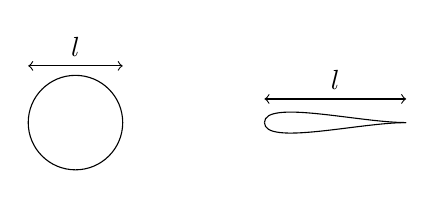
\begin{tikzpicture}[scale=0.6]
        \draw (0,0) circle(1);
        \draw [<->] (-1,1.2) -- (1,1.2);
        \draw (0,1.2) node[above] {$l$};
        \draw (4,0) ..controls +(0,0.5) and +(-1,0).. (7,0);
        \draw (4,0) ..controls +(0,-0.5) and +(-1,0).. (7,0);
        \draw [<->] (4,0.5) -- (7,0.5);
        \draw (5.5,0.5) node[above] {$l$};
    \end{tikzpicture}
\end{center}
%
Pour un écoulement dans une conduite (dit \textit{interne}), on utilise souvent le \textit{diamètre hydraulique}. Il est défini par $D_h = 4 \cdot S/P$ avec $S$ la surface transverse à l'écoulement et $P$ le périmètre de cette surface. Pour un tuyau, il correspond à son diamètre (logique). Pour une conduite en anneau, il vaut la différence des diamètres extérieur et intérieur de l'anneau.

Pour un écoulement dans une conduite circulaire, les nombres de Reynolds limites ont été précisément identifiés par expérience :
\begin{itemize}
    \item régime laminaire : $Re<2100$
    \item régime turbulent : $Re>4000$
\end{itemize}
